%-----------------------------------------------------------------------------
%	 Placas Programables
%-----------------------------------------------------------------------------

\lhead[\thepage]{Placas Programables \thechapter. \rightmark}
\rhead[Placas Programables \thechapter. \leftmark]{\thepage}

%	Capitulo 5: Placas Programables
\chapter{Placas Programables}
\markboth{Placas Programables}{Placas Programables}

%	Sección uno: Definición
\section{Definición}
\lhead[\thepage]{\thesection. Definición}
Las placas programables, también llamadas placas de programación o desarrollo son dispositivos básicos que cuentan con un microcontrolador programable con el cual se pueden ejecutar diferentes instrucciones. En muchos escenarios estamos en presencia de una computadora de recursos muy reducidos (conocidos como Single Board Computer o SBC por sus siglas en inglés), pues siguen al pie de la letra con la arquitectura del computador de John von Nuemann\cite{arquitecturaComputador}.\\ 

Estas computadoras de una sola placa se hicieron como sistemas de demostración o desarrollo, para sistemas educativos o para su uso como controladores integrados de computación los que las hace especialmente útiles para poder crear prototipos funcionales de dispositivos de toda clase, desde robots hasta dispositivos de Internet de las cosas. Para poder crear las rutinas se hacen uso de lenguajes de programación que establecen el control directo contra la microprocesador o incluso contra los sensores y actuadores que puedan estar conectados al dispositivo.\\

Algunas placas incluso poseen la capacidad de soportar un sistema operativo completo los cuales los hacen inmensamente flexibles a la hora de realizar tareas, de agregar nuevos sensores o controlar otros dispositivos a través de esa placa. Existen gran cantidad de modelos distintos en el mercado. Sin embargo en este trabajo de investigación nos centraremos en dos tipos de placas en específico:

%	Sección dos: Placas Arduino
\section{Placas Arduino}
\lhead[\thepage]{\thesection. Placas Arduino}
Arduino (Genuino a nivel internacional es una plataforma electrónica en hardware y software libres, fáciles de usar. Está pensado para cualquier persona que haga proyectos interactivos.\cite{ArduinoOfficial}(figura \ref{fig:arduino_logo}) Las placas Arduino tiene la capacidad  detectar el ambiente recibiendo entradas de variedad de sensores, y afecta su entorno controlando luces, motores y otros actuadores. La lógica de micro controlador Arduino deberá hacerse escribiendo código en el lenguaje de programación Arduino (basado en C++) y utilizando el entorno de desarrollo de Arduino.\\

\begin{figure}[htb]
\centering
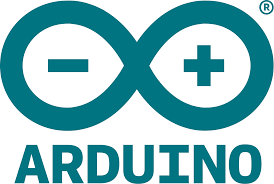
\includegraphics[scale=0.35]{./Figuras/arduino_logo.png}
\caption{Logo del proyecto Arduino}
\label{fig:arduino_logo}
\vspace*{-10pt}
\end{figure}

Arduino nació en el Ivrea Interaction Design Institute como una herramienta fácil para el prototipado rápido, dirigido a estudiantes sin formación en electrónica y programación. Tan pronto como llegó a una comunidad más amplia, la junta de Arduino comenzó a cambiar para adaptarse a las nuevas necesidades y desafíos, diferenciando su oferta de simples placas de 8 bits a productos para aplicaciones IoT, portátiles, impresión 3D y dispositivos embebidos. Todas las placas de Arduino son totalmente de hardware libre, lo que permite a los usuarios construirlas independientemente y eventualmente adaptarlas a sus necesidades particulares. El software, también es de código abierto y está creciendo a través de las contribuciones de los usuarios de todo el mundo.\\

Las placas Arduino están disponibles de dos formas: ensambladas o en forma de kits ``Hágalo tú mismo''. Los esquemas de diseño del hardware están disponibles bajo licencia Libre, con lo que se permite que cualquier persona pueda crear su propia placa Arduino sin necesidad de comprar una prefabricada. La primera placa Arduino fue introducida en 2005 llamada Arduino Uno \ref{fig:arduinouno}), ofrecida a un bajo costo y facilidad de uso para novatos y profesionales. Se buscaba desarrollar proyectos interactivos con su entorno mediante el uso de actuadores y sensores. A partir de octubre de 2012, se incorporaron nuevos modelos de placas de desarrollo que usan micro controladores Cortex M3, ARM de 32 bits, que coexisten con los originales modelos que integran micro controladores AVR de 8 bits.\\

En la actualidad, existen 29 distintas placas de micro controladores, 7 módulos complementarios, 15 Shields (placas de expansión), con lo cual se posee un ecosistema rico de diversos micro controladores para cada tarea o cada ambiente de desarrollo. 

\begin{figure}[htb]
\centering
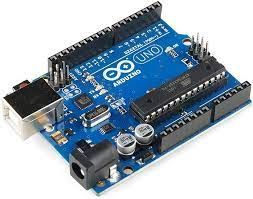
\includegraphics[scale=0.7]{./Figuras/arduino_uno.jpeg}
\caption{Arduino Uno R3}
\label{fig:arduinouno}
\vspace*{-10pt}
\end{figure}

%	Sección tres: Placas Raspberry Pi
\section{Placas Raspberry Pi}
\lhead[\thepage]{\thesection. Placas Raspberry Pi}
Raspberry Pi es una marca (figura \ref{fig:raspi_logo}) de micro computadores de hardware libre, que comenzó como proyecto para llevar a la educación  de escolares ingleses conceptos de la computación, de la programación y de la electrónica, y que luego la comunidad Maker y algunas compañías adoptaron, pues vieron el potencial para crear dispositivos, sensores, actuadores, robots entre otros y para poder llevar a cabo prototipos funcionales de dispositivos y de productos muy rápidamente. El relativo bajo costo (que va desde \$10 por la placa mas sencilla hasta \$80 por el modelo más avanzado) y facilidad de uso, han facilitado la adopción de este micro computador por personas en todo el mundo para toda clase de proyectos amateurs y profesionales.

\begin{figure}[htb]
\centering
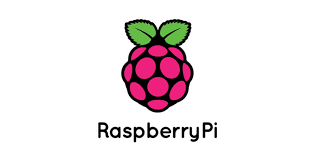
\includegraphics[scale=0.65]{./Figuras/raspi_logo.png}
\caption{Logo de la marca Raspberry Pi}
\label{fig:raspi_logo}
\vspace*{-10pt}
\end{figure}

Este es un proyecto llevado a cabo con la Raspberry Pi Foundation\cite{RaspberryPi} desde el año 2012 ofreciendo hasta el día de hoy siete modelos distintos de placas, con procesadores ARM, memoria RAM que va desde los 256MB hasta 1GB y cuya memoria es de carácter externo usando tarjetas MicroSD en la mayoría de los modelos y cuyo consumo no es mayor al de 2,5 amperios. Los modelos son:
\begin{itemize}
\item Raspberry Pi Modelo A: Fue el primer modelo de Raspberry Pi en salir al mercado, en el año 2012. Basado en un SoC Broadcom BCM28235, cuyo procesador es un ARM11 32 bits a 700MHz, Gráficas Broadcom VideoCore IV, con 256MB de memoria RAM, un puerto USB, una salida HDMI, un conector RCA, una entrada CSI para un modulo de cámara, y sin características de conectividad alguna por defecto. Para el almacenamiento se usan tarjetas SD. 
\item Raspberry Pi Modelo B/B+: También del año 2012, es una variante del Modelo A, trajo consigo diversas mejoras, como la inclusión del doble de memoria RAM, pasando de 256MB a 512MB. Trajo consigo un puerto USB más y un conector Ethernet (RJ-45) Se mantuvo tanto su tamaño como su coste. No hubo variaciones en el procesador ni en la gráfica. Tiempo después se lanzo el Modelo B+, que incluyó 4 puertos USB y pasó de usar una SD a una MicroSD.
\item Raspberry Pi 2 Modelo B: Lanzada en 2014 es el primer modelo que no incluye el mismo procesador usado en los tres anteriores: se sustituye por uno de la misma marca, pero de modelo BCM2836 con lo cual pasa de ser de un núcleo a cuatro, y de 700MHz a 900MHz, no obstante emplea la misma gráfica, la VideoCore IV. Dobla la cantidad de memoria RAM, pasando de 512MB a 1GB de memoria (también compartida con la gráfica). También incluye 40 pines GPIO, y mantiene los cuatro puertos USB. Suprime la conexión RCA.
\item Raspberry Pi 3 Modelo B: Sale al mercado en el año 2016, renovando procesador, una vez más de la compañía Broadcom, siendo un procesador de cuatro núcleos al igual que el modelo anterior, pero pasa de 900MHz a 1.20GHz,  manteniendo la RAM en 1GB. Su mayor novedad fue la inclusión de WiFi y Bluetooth (4.1 Low Energy) sin necesidad de adaptadores.
\item Raspberry Pi Zero: Fue el primer modelo miniaturizado de las Raspberry Pi, teniendo un tamaño un poco mayor a un Pen Drive. Lanzado en 2015 con un coste de 5 dólares, es una 40\% más potente que el primer modelo de Raspberry. Tiene un CPU Broadcom BCM2835, que funciona a 1GHz con dos núcleos. Posee 512MB de RAM, y comparte la gráfica VideoCore IV. Debido a su tamaño sustituye el puerto HDMI por MiniHDMI, manteniendo así las prestaciones. Tampoco usa USB estándar, sino que tiene dos MicroUSB, uno de alimentación y otro de datos. Posee salida RCA, pero en vez de por clavija son solo dos conectores integrados en la placa. Usa MicroSD como sistema de almacenamiento.(figura \ref{fig:rpizero})

\begin{figure}[htb]
\centering
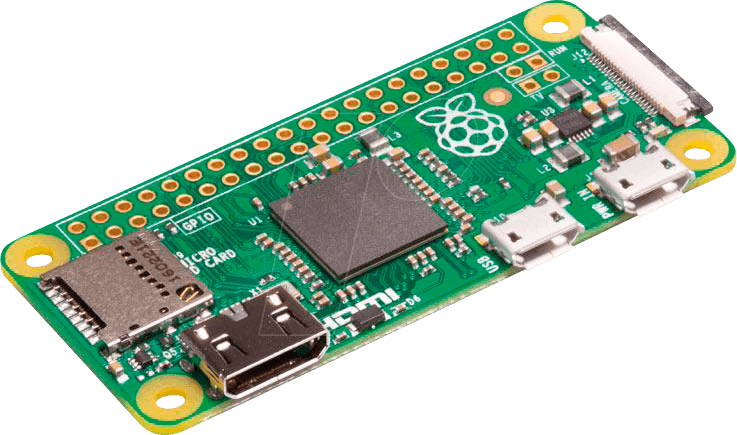
\includegraphics[scale=0.25]{./Figuras/rpizero.png}
\caption{Raspberry Pi 4 modelo B}
\label{fig:rpizero}
\vspace*{-10pt}
\end{figure}

\item Raspberry Pi Zero W: Es la sucesora de la Raspberry Pi Zero. la W es por Wireless, ya que la única novedad de esta placa con respecto a su antecesora es la inclusión de WiFi y Bluetooth, por lo que su precio ascendió a 11 dólares.
\item Raspberry Pi 3 Modelo B+: Del mismo modo que para el Raspberry Pi Modelo B, esta es una actualización en términos de rendimiento sobre la Raspeberry Pi 3 Modelo B. Pasa a ser un poco más rápida que su antecesora y ofrece la capacidad de conectarse a Wifi doble banda. Incorpora Bluetooth 4.2 y la velocidad de su puerto ethernet pasa de 100 Mbits/seg a 300 Mbits/seg.
\item Raspberry Pi 3 Modelo A:  Los modelos A+ presentan menores prestaciones a un menor precio. Cuenta con 512 MB de RAM (compartidos con la GPU VideoCore IV), un solo puerto USB y sin puerto de conexión de red ethernet.
\item Raspberry Pi 4 modelo B: Esta versión viene a sustituir a la versiones 3 y cambia los puertos HDMI de tamaño completo por dos puertos microHDMI. Cuenta con la capacidad de manejar una pantalla a 4K a 60 Hz, o dos pantallas 4K a 30 Hz. Se ha incluido por primera vez USB 3.0, y el puerto Ethernet ya no está limitado a 300 Mbps. Tiene un procesador Broadcom nuevo. Es la primera serie que posee 3 variantes disponibles en los que cambia la cantidad de memoria RAM de 2GB, 4GB, y de 8GB (figura \ref{fig:rpi4}).

\begin{figure}[htb]
\centering
\includegraphics[scale=0.05]{./Figuras/rpi4.jpg}
\caption{Raspberry Pi 4 modelo B}
\label{fig:rpi4}
\vspace*{-10pt}
\end{figure}

\item Raspberry Pi 400: Cuenta con una placa personalizada que se deriva de la Raspberry Pi 4 existente, específicamente remodelada para incluirla en un teclado derivado del Raspberry Pi Keyboard. Posee una solución de enfriamiento mas robusta que su contraparte 4 modelo B al poseer una placa de metal ancha para disipar el calor y un conmutador actualizad para la fuente de alimentación que es un poco mas alta que la del Raspberry Pi 4. La computadora cuenta con 4GB de memoria RAM LPDDR4.
\item Raspberry Pi Pico: Anunciada en el 2021, es una placa pequeña y versátil construida con RP2040, un nuevo chip microcontrolador diseñado por Raspberry Pi Fundation. Este modelo está gobernada por un pequeño SoC que cuenta con un procesador dual core ARM Cortex M0+ funcionando a 133 MHz, acompañado de 264 KB de RAM y 2 MB de almacenamiento integrado.
\item Raspberry Pi 5: La mas nueva de las versiones del Raspberry Pi existentes al momento de la escritura de esta investigación representa el salto de rendimiento sobre el modelo anterior de Raspberry Pi 4. Con un procesador  Broadcom BCM2712 casi duplica la frecuencia del CPU con respecto a su predecesora, además de contar ahora con una nueva GPU VideoCore VII mucho más rápida con una frecuencia de 800 MHz. Entre otras mejoras.
\end{itemize}
Existen gran variedad de sistemas operativos que pueden ser usados con este micro computador, la mayoría de ellos, basados en Linux, pero también con la posibilidad de instalar Windows 10 (Iot Core) o Android (Android Things).\\

Una característica principal de estas placas es la existencia de 40 pines GPIO, los cuales proveen entradas y salidas digitales para el micro computador con lo que se le puede expandir su s funcionalidades con el uso de sensores (HATs o a través de circuitos eléctricos tradicionales), cuya lógica puede ser creada en lenguajes de programación como Python, C++, Java, entre otros.\\

El proyecto ha ganado una comunidad muy amplia alrededor del mundo, que han probado la versatilidad que posee este micro computador en proyectos de toda índole, dando a las personas la capacidad de crear soluciones basadas en IoT con una relación coste-rendimiento positivo.

